\paragraph{QuizziPedia::Front-End::ModelViews::StringsSortingQuestionsModelView}
\begin{figure} [ht]
	\centering
	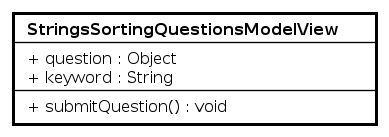
\includegraphics[scale=0.80]{UML/Classi/Front-End/QuizziPedia_Front-end_ModelView_StringsSortingQuestionsModelView.png}
	\caption{QuizziPedia::Front-End::ModelViews::StringsSortingQuestionsModelView}
\end{figure} \FloatBarrier
\begin{itemize}
	\item \textbf{Descrizione}: classe di tipo modelview la cui istanziazione è contenuta all'interno della variabile di ambiente \$scope di \textit{Angular.js\ped{G}}. All'interno di essa sono presenti le variabili e i metodi necessari per il \textit{Two-Way Data-Binding\ped{G}} tra la view \texttt{StringsSortingQuestionsView} e il controller \texttt{StringsSortingQuestionsController}; 
	\item \textbf{Utilizzo}: viene utilizzata per effettuare il \textit{Two-Way Data-Binding\ped{G}} tra la view \texttt{StringsSortingQuestionsView} e il controller \texttt{StringsSortingQuestionsController} rendendo disponibili variabili e metodi;
	\item \textbf{Relazioni con altre classi}:
	\begin{itemize}
		\item \textit{IN} \texttt{StringsSortingQuestionsView}: view contenente i campi e le direttive per creare una domanda a ordinamento stringhe; 
		\item \textit{IN} \texttt{StringsSortingQuestionsController}: questa classe permette di gestire la creazione e la modifica di una domanda a ordinamento di stringhe;
	\end{itemize}
	\item \textbf{Attributi}:
	\begin{itemize}
			\item \texttt{+ question: Object} \\ Oggetto contenente gli attributi per la creazione della domanda:
			\begin{itemize}
				\item \texttt{answer}: array contenente oggetti che rappresentano le risposte. Ogni oggetto risposta contiene:
				\begin{enumerate}
					\item \texttt{textSorting}: attributo di tipo \texttt{String} che contiene il testo della risposta;
					\item \texttt{position}: attributo di tipo \texttt{Number} che indica la giusta posizione del testo.
				\end{enumerate}
			\end{itemize}
			\item \texttt{+ keyword: String} \\ Attributo contenente la keyword associata alla domanda/questionario;	  
	\end{itemize}
	\item \textbf{Metodi}:
	\begin{itemize}
		\item \texttt{+} \texttt{submitQuestion(): void}\\ 
		Metodo che gestisce l’evento click sul pulsante di conferma sulla domanda. Raccoglie i dati dal modelview e li manda al server attraverso \texttt{QuestionService}. Poi verrà effettuato il redirect alla pagina di gestione delle domande oppure al questionario che si stava creando; 
	\end{itemize}
\end{itemize}

